\documentclass[Afour,sagev,times,doublespace]{sagej}

\usepackage{amsmath}
\usepackage{booktabs}
\usepackage{graphicx}
\usepackage[colorlinks,bookmarksopen,bookmarksnumbered,citecolor=blue,urlcolor=blue]{hyperref}

\def\volumeyear{2026}

\begin{document}

\runninghead{Walther et al.}

\title{Sampling Design for Spatial Cluster Randomized Trials Under Heterogeneous Incidence}

\author{Andrew Walther\affilnum{1}, Ross Joseph Simpson, Jr.\affilnum{2}, Ashkan Habib\affilnum{1}, and Feng-Chang Lin\affilnum{1}}

\affiliation{\affilnum{1}Department of Biostatistics, University of North Carolina at Chapel Hill, Chapel Hill, NC, USA\\
\affilnum{2}Division of Cardiology, University of North Carolina School of Medicine, Chapel Hill, NC, USA}

\corrauth{Andrew Walther, Department of Biostatistics, University of North Carolina at Chapel Hill, Chapel Hill, NC 27599, USA.}

\email{awalther@unc.edu}

\begin{abstract}
\textbf{Background/Aims:} Spatial cluster randomized trials (CRTs) are vulnerable to bias from spatial spillover, in which treatment effects diffuse from treated to nearby control clusters, and from spatial dependence in the outcome itself. Existing spillover-mitigation methods are almost entirely analysis-stage corrections applied after data collection. We evaluated whether the choice of treatment assignment design, fixed before a trial begins, can reduce estimation error under spillover without requiring any post-hoc adjustment.

\textbf{Methods:} We simulated a 100-cluster spatial grid with outcomes generated from a spatial Durbin model incorporating a spillover term and spatially autocorrelated residual dependence. Baseline outcome incidence was generated under three heterogeneity mechanisms (independent, spatially clustered, and population-scaled Poisson) and used to inform incidence-aware designs. Six treatment assignment strategies, representing three conceptually distinct mechanisms of spillover control (a saturation approach, a buffering/isolation approach, and two incidence-stratified balancing approaches), plus a spatial-separation strategy and a spatial blocking strategy, were compared. The true direct treatment effect was swept across five magnitudes. Each design--parameter combination was replicated under 320 spatial and spillover parameter configurations, with maximum likelihood spatial regression as the estimator throughout. Formal non-parametric hypothesis testing (Friedman and Nemenyi tests) compared mean squared error (MSE) ranks across designs.

\textbf{Results:} An incidence-guided saturation design, which varies treatment saturation across spatial regions in proportion to historical incidence, achieved the lowest MSE (0.079) and near-nominal 95\% confidence interval coverage (94\%). A design that maximizes spatial separation between treated and control clusters (checkerboard-style alternation) performed worst by a wide margin (MSE 0.802) and its coverage collapsed to 53\%, meaning its confidence intervals missed the true effect roughly half the time. The MSE ranking of designs was stable across all five treatment-effect magnitudes tested (Friedman $\chi^2$ range 557.3--800.9, all $p<2.2\times10^{-16}$). A preliminary application-scale illustration, using synthetic placeholder incidence over North Carolina's Community College service-area network as candidate clusters for a planned sudden unexpected death (SUD) prevention pilot, showed a qualitatively consistent pattern favoring incidence-stratified and saturation-based designs.

\textbf{Conclusions:} Incidence-informed saturation designs can materially reduce estimation error and preserve valid inference under spatial spillover, while maximal spatial separation, a design intuition borrowed from non-spatial CRT practice, is actively harmful when spillover is present. These findings support incorporating spatial spillover structure into the design stage of cluster randomized trials, ahead of statistical modeling choices made after data collection. Application to a real SUD surveillance dataset, currently in preparation, is needed before a design recommendation for that setting can be finalized.
\end{abstract}

\keywords{cluster randomized trial, spatial interference, spillover, treatment assignment, spatial autocorrelation, simulation study, trial design}

\maketitle

\section{Introduction}

Cluster randomized trials (CRTs) randomize intact groups, such as clinics, schools, or geographic areas, rather than individuals, and are the standard design when an intervention is delivered at the group level or when individual randomization would create unacceptable contamination.\cite{donner_design_2000,hayes_cluster_2017} A central assumption underlying standard CRT analysis is the stable unit treatment value assumption (SUTVA): a control cluster's outcome must not depend on which other clusters were treated.\cite{hudgens_toward_2008} This assumption is routinely violated when clusters are spatially arranged. Tobler's first law of geography, that near things are more related than distant things, implies that an intervention delivered in one location can plausibly influence outcomes in geographically adjacent locations through shared populations, service networks, information diffusion, or environmental pathways.\cite{tobler_computer_1970} Documented examples of such spatial spillover span infectious disease control, where treating one household reduces transmission risk in neighboring households,\cite{binka_impact_1998} and deworming interventions, where treated schools reduce infection prevalence at nearby untreated schools.\cite{miguel_worms_2004} When spillover is present but unmodeled, standard CRT estimators are biased, and the direction and magnitude of that bias depend on the spatial arrangement of treated and control clusters.

The methodological literature on spatial interference has concentrated on analysis-stage correction: detecting spillover using spatial autocorrelation statistics after outcomes are observed,\cite{moran_interpretation_1948,geary_contiguity_1954} and fitting spatial regression models such as the spatial Durbin model to separate direct and spillover effects post hoc.\cite{ord_estimation_1975,bivand_r_2022} Design-stage mitigation, choosing a treatment assignment strategy before randomization that limits spillover's ability to bias estimation in the first place, has received comparatively little attention. Jarvis et al. reviewed the sparse literature on spatial CRT design and highlighted this gap explicitly.\cite{jarvis_spatial_2017} Covariate-constrained randomization offers one partial design-stage tool, balancing measured covariates across arms to reduce confounding,\cite{crisp_covariate-constrained_2023} building on earlier work on balance in cluster randomized trials,\cite{raab_balance_2001} but it was not developed with spatial spillover specifically in mind. A cluster of recent work is now converging on this exact problem: randomized saturation designs deliberately vary treatment intensity across units to identify both direct and spillover effects,\cite{baird_optimal_2018} fried-egg and buffer-zone designs used in malaria trials leave an untreated ring around treated clusters to limit contamination,\cite{mccann_spatial_2018} and a growing theoretical literature has derived rate-optimal cluster designs and independent-set designs explicitly under network and spatial interference.\cite{leung_rateoptimal_2022,cai_independentset_2023,leung_clusterrandomized_2025,watson_design_2025} This body of work signals that the field is actively moving toward design-stage solutions, but it has not yet produced a systematic, simulation-based comparison of design strategies under realistic, heterogeneous spatial conditions.

This paper extends an earlier proof-of-concept study, which compared simple random assignment against a single block-stratified design on small, exhaustively enumerable grids (8--12 clusters) and estimated a structural spatial Durbin model with separate parameters for baseline, direct, spillover, and dependence effects. That prior work's own discussion explicitly anticipated the need for a larger design space and for heterogeneous, rather than uniform, baseline outcome risk. This paper answers that call: we scale to a 100-cluster grid, compare six conceptually distinct treatment assignment strategies rather than two, and generate baseline incidence under three heterogeneity mechanisms so that some designs can exploit prior knowledge of spatial risk while others cannot.

Our aims are threefold: (1) to rank the six designs by estimation accuracy (mean squared error, MSE) and inferential validity (95\% confidence interval coverage) within each incidence-generating mechanism; (2) to test whether that ranking is stable across the spatial and spillover parameters a trial team cannot control in advance, including the magnitude of the true treatment effect; and (3) to translate the ranking into concrete design guidance, illustrated using a real, currently developing application: a planned sudden unexpected death (SUD) prevention pilot delivered through North Carolina's community college network. The remainder of this paper describes the simulation methods, reports the design comparison results, presents the SUD application context, and discusses implications and limitations.

\section{Methods}

\subsection{Spatial structure and outcome model}

We simulated a $10\times10$ regular grid of 100 clusters, with adjacency defined by queen contiguity (clusters sharing an edge or corner are neighbors). A row-standardized spatial weights matrix $W$ was constructed from this adjacency structure. Cluster-level outcomes $Y$ were generated from a spatial Durbin model,
\begin{equation}
Y = (I - \rho W)^{-1}\left[\tau Z + \gamma W Z + \beta X + \epsilon\right], \quad \epsilon \sim N(0, \sigma^2 I),
\end{equation}
where $Z$ is the binary treatment assignment vector, $\tau$ is the direct treatment effect of interest, $\gamma$ is the spillover coefficient governing how much a cluster's outcome is influenced by the treatment status of its neighbors ($WZ$), $\rho$ is the spatial autoregressive coefficient governing residual dependence in the outcome itself, $X$ is a baseline incidence covariate with fixed coefficient $\beta=1$, and $\sigma=1$. Spillover was evaluated under two exposure regimes: one in which spillover accrues to control clusters only (as in classic contamination), and one in which it accrues to both treated and control clusters (as when neighboring effects reinforce treatment). All simulation code, exact parameter grids, and reproducibility details are provided in the online supplementary material.

\subsection{Heterogeneous baseline incidence}

Unlike a setting with uniform baseline risk, real cluster-level health outcomes vary spatially in ways that a trial team may or may not be able to observe in advance. We generated baseline incidence $X$ under three mechanisms: independent and identically distributed noise (no spatial structure), spatially autocorrelated incidence generated from the same spatial process as the outcome model at two autocorrelation strengths, and a population-scaled Poisson count process calibrated to a sudden-death base rate of 35 per 100{,}000 (motivated by our applied setting, described below). Incidence was generated once per configuration and held fixed across replications of a given design; only the first replication's ``observed'' incidence was made available to incidence-aware designs, mimicking how a trial team would use historical surveillance data rather than the true underlying risk surface.

\subsection{Treatment assignment designs}

We compared six treatment assignment designs, each representing a conceptually distinct strategy for limiting spillover-induced bias (Table~\ref{tab:designs}). Two designs are deterministic given the incidence surface (Checkerboard and High Incidence Focus) and were generated once and held fixed; the remaining four were re-randomized for each replication. Two additional designs evaluated in the underlying simulation study, plain saturation quadrants and a two-strata (median-split) balancing design, were dropped from this comparison because they were statistically indistinguishable from a retained design that implements the same mechanism with an incidence-informed refinement (Nemenyi $p=1.00$ for saturation quadrants versus its incidence-guided counterpart; lower MSE and finer stratification for balanced quartiles versus the median-split variant). The complete eight-design comparison, including these two variants, is reported in the online supplementary material.

\begin{table*}[t]
\small\sf\centering
\caption{The six treatment assignment designs compared, ordered by mean squared error at the primary treatment-effect magnitude ($\tau=1.0$; see Table~\ref{tab:results}). ``Deterministic'' designs use the same assignment for every simulation replicate within a scenario.\label{tab:designs}}
\begin{tabular}{p{4.2cm}p{9.2cm}p{1.5cm}p{1.8cm}}
\toprule
Design & Targeting logic & \% treated & Deterministic \\
\midrule
Incidence-Guided Saturation Quadrants & Spatial quadrants receive a randomized saturation level (20--80\% treated within quadrant), assigned in rank order of quadrant-average incidence & $\sim$50 & No \\
Balanced Quartiles & Clusters stratified into incidence quartiles; 1:1 randomization within each quartile & $\sim$50 & No \\
High Incidence Focus & Top 50\% of clusters by observed incidence are treated & 50 & Yes \\
Isolation Buffer & Greedy assignment such that no two treated clusters are spatially adjacent & 20--30 & No \\
2$\times$2 Blocking & Grid partitioned into 2$\times$2 spatial blocks; 1:1 randomization within each block & 50 & No \\
Checkerboard & Alternating assignment across the grid, maximizing spatial separation between treated and control clusters & 50 & Yes \\
\bottomrule
\end{tabular}
\end{table*}

\subsection{Estimation}

The direct treatment effect $\tau$ was estimated using maximum likelihood spatial regression (\texttt{lagsarlm}) fit to a spatial Durbin specification matching the outcome-generating model, including the true spillover exposure term as a covariate. This oracle specification represents a best-case bound on estimation performance and is discussed as a limitation below.

\subsection{Simulation design and metrics}

The parameter space combined five incidence configurations (independent, two spatial-incidence strengths, two Poisson strengths), two neighbor definitions, four levels of outcome spatial dependence $\rho$, four levels of spillover magnitude $\gamma$, two spillover exposure regimes, the six designs above, and five true treatment-effect magnitudes ($\tau \in \{0.8, 1.0, 1.5, 2.0, 3.0\}$), totaling 9{,}600 scenarios for the six-design comparison (12{,}800 across all eight designs). Each scenario was replicated 25 times over treatment assignment and 10 times over outcome draws (250 total iterations), except the two deterministic designs, which were replicated only over outcome draws. We report bias, standard deviation, MSE, 95\% confidence interval coverage, and statistical power to reject a null direct effect of zero. Exact resample counts, the full parameter grid, and metric formulas are given in the online supplementary material.

\section{Results}

\begin{table}[h]
\small\sf\centering
\caption{Mean squared error and 95\% confidence interval coverage by design at the primary treatment-effect magnitude ($\tau=1.0$), averaged over 320 spatial and spillover parameter configurations. Friedman rank-sum test: $\chi^2=800.9$, $\mathrm{df}=5$, $p<2.2\times10^{-16}$. Nemenyi post-hoc comparisons found 13 of 15 pairwise design comparisons statistically significant at $\alpha=0.05$.\label{tab:results}}
\begin{tabular}{lcc}
\toprule
Design & MSE & Coverage \\
\midrule
Incidence-Guided Saturation Quadrants & 0.079 & 0.941 \\
Balanced Quartiles & 0.102 & 0.938 \\
High Incidence Focus & 0.133 & 0.966 \\
Isolation Buffer & 0.148 & 0.939 \\
2$\times$2 Blocking & 0.228 & 0.937 \\
Checkerboard & 0.802 & 0.527 \\
\bottomrule
\end{tabular}
\end{table}

Incidence-Guided Saturation Quadrants achieved the lowest MSE (0.079) with coverage close to the nominal 95\% level (94\%), followed by Balanced Quartiles (MSE 0.102), High Incidence Focus (MSE 0.133), Isolation Buffer (MSE 0.148), and 2$\times$2 Blocking (MSE 0.228); all four maintained coverage between 93\% and 97\% (Table~\ref{tab:results}, Figure~\ref{fig:mse}). Checkerboard, the design that maximizes spatial separation between treated and control clusters, performed worst by a wide margin (MSE 0.802) and its confidence interval coverage collapsed to 53\% (Figure~\ref{fig:coverage}), meaning the nominal 95\% interval failed to contain the true treatment effect roughly half the time. This is a design-induced inferential failure, not merely a loss of precision: maximizing distance between treated and control units, an intuition carried over from non-spatial CRT practice, concentrates spillover exposure asymmetrically across the grid in a way that a maximum likelihood spatial model estimating a single global $\tau$ cannot fully correct.

High Incidence Focus, while competitive in mean MSE, showed the largest cross-configuration variability of the top five designs (MSE ranging from 0.078 to 0.207 depending on the incidence-generating mechanism), because its performance is entirely contingent on how informative the observed incidence surface is; when historical incidence poorly reflects the true underlying risk surface, targeting the wrong half of the grid can approach the separation problem that degrades Checkerboard.

This ranking was stable across all five tested treatment-effect magnitudes. The omnibus Friedman test rejected equal design ranks at every level of $\tau$ (Figure~\ref{fig:tau}; $\chi^2 = 730.6$, $800.9$, $705.7$, $658.5$, and $557.3$ for $\tau = 0.8, 1.0, 1.5, 2.0, 3.0$ respectively; all $p<2.2\times10^{-16}$), indicating that the relative advantage of incidence-informed and buffering designs over Checkerboard does not depend on the size of the true effect being detected.

\begin{figure}[h]
\centering
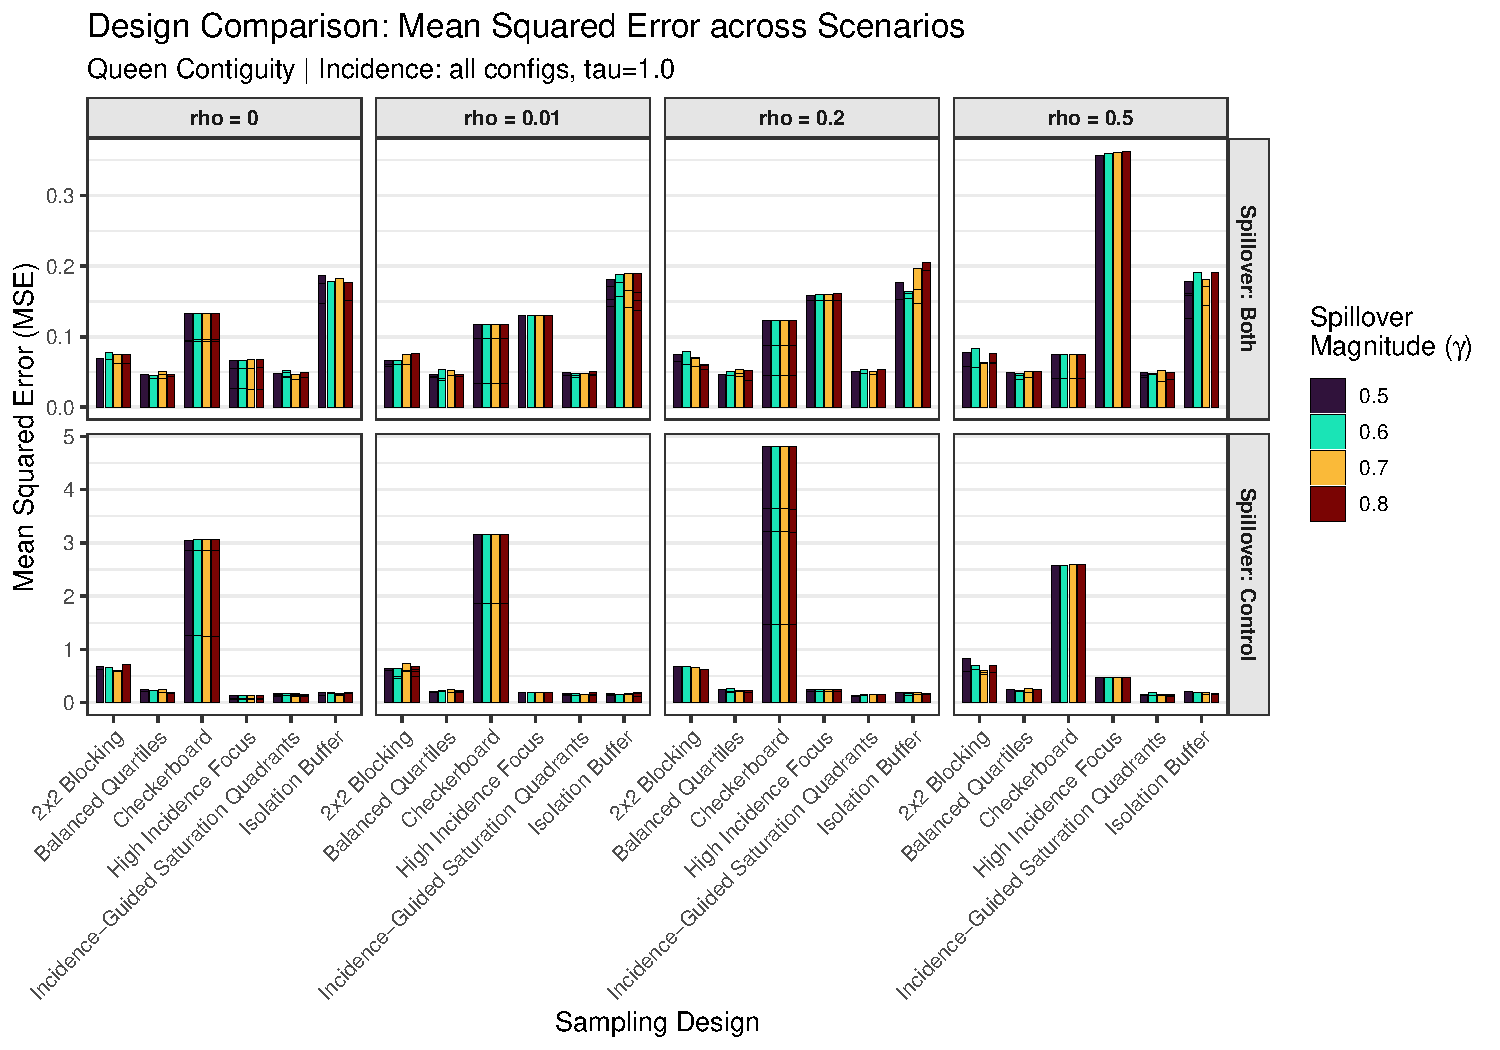
\includegraphics[width=0.95\linewidth]{figures/fig_mse_by_design_6design.pdf}
\caption{Mean squared error by design and spillover exposure regime, at the primary treatment-effect magnitude ($\tau=1.0$), faceted by outcome spatial dependence $\rho$ and spillover exposure regime.\label{fig:mse}}
\end{figure}

\begin{figure}[h]
\centering
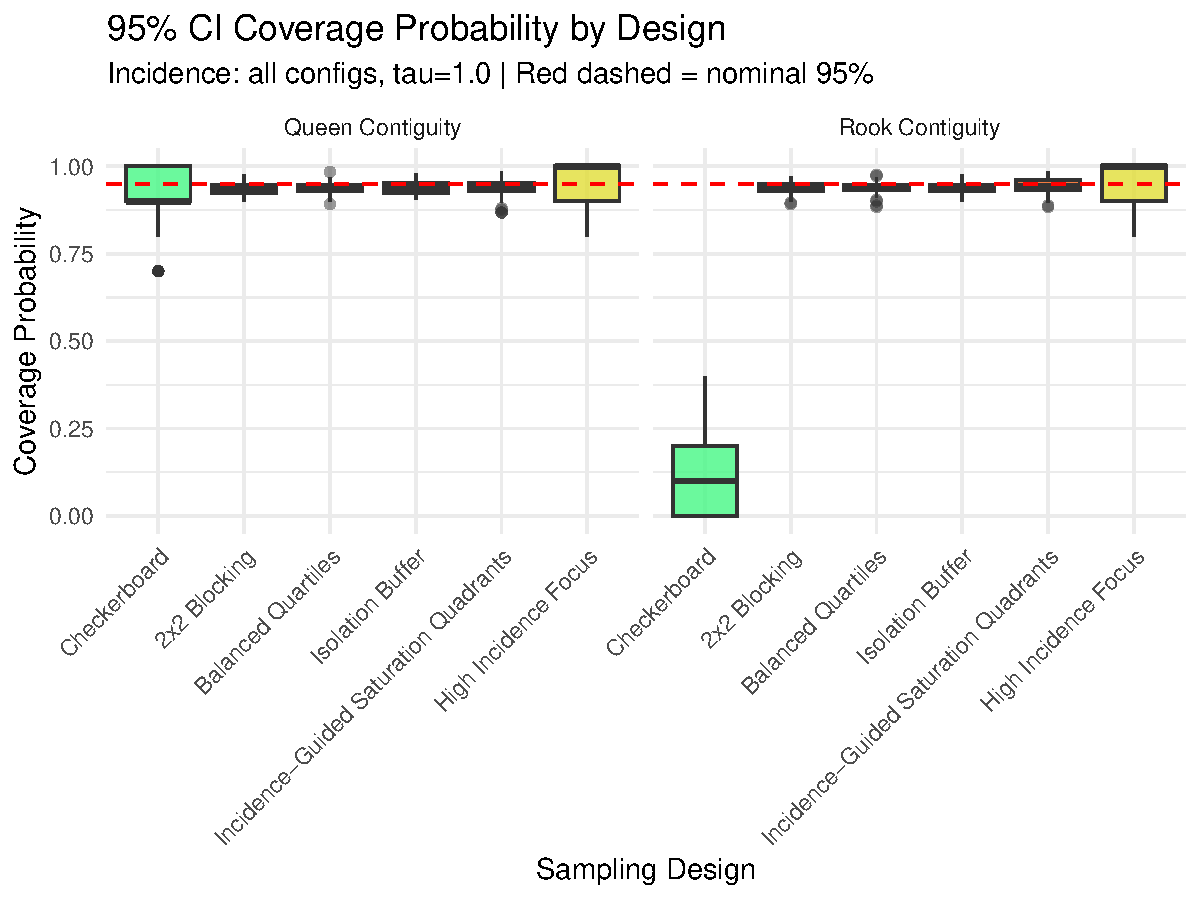
\includegraphics[width=0.8\linewidth]{figures/fig_coverage_by_design_6design.pdf}
\caption{95\% confidence interval coverage by design at $\tau=1.0$. The dashed red line marks the nominal 95\% level.\label{fig:coverage}}
\end{figure}

\begin{figure}[h]
\centering
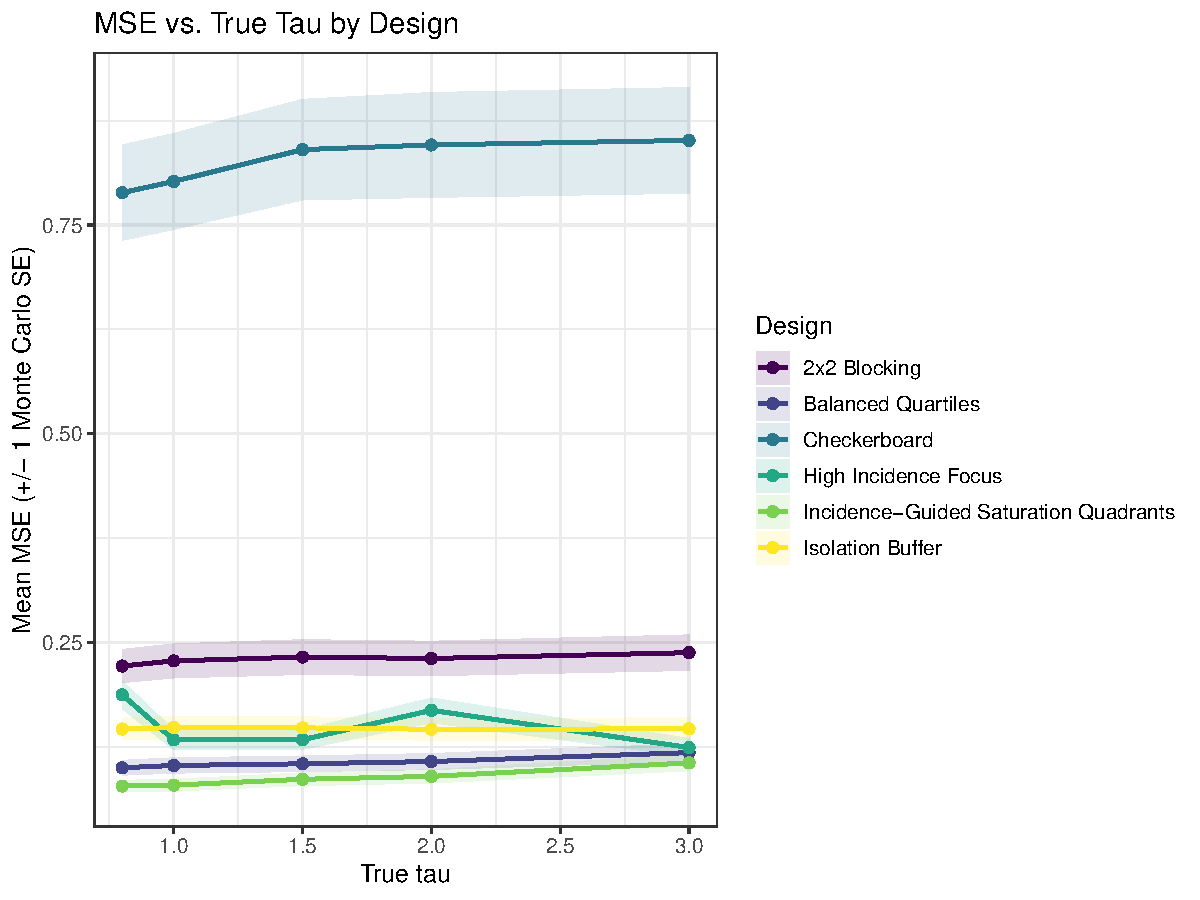
\includegraphics[width=0.8\linewidth]{figures/fig_tau_sensitivity_6design.pdf}
\caption{Mean squared error by design across the five tested treatment-effect magnitudes.\label{fig:tau}}
\end{figure}

\section{Application: A Planned Sudden Unexpected Death Prevention Pilot in North Carolina}

Sudden unexpected death (SUD) in adults is a substantial, incompletely understood cause of premature mortality; a validated death-certificate classification algorithm (SUDDEN) has been used to estimate a North Carolina base rate near 35 per 100{,}000, with productivity loss from SUD in working-age adults exceeding that of any individual cancer,\cite{mirzaei_years_2019} and documented geographic and socioeconomic gradients, including elevated incidence in rural counties\cite{gan_factors_2019} and an inverse relationship with household income in Wake County.\cite{mounsey_relation_2017}

A pilot intervention is being planned in collaboration with North Carolina's community college (CC) system, which offers a natural spatial and organizational unit for this design framework. North Carolina's 58 community colleges collectively serve all 100 counties, with a primary campus in one county and satellite campuses in neighboring counties (for example, Durham Technical Community College also operates a campus in Orange County); this network structure is a direct, real-world analog to the spillover mechanism modeled in this paper, because CCs communicate and coordinate with one another. The planned pilot site is Lenoir County Community College, with anticipated spillover to its Kinston and Jones County satellite sites. Because the teaching intervention under consideration is delivered county-wide rather than at finer spatial resolution, the natural treatment unit is the CC service area rather than the census tract. Real SUD incidence data for this application, classified from approximately 100{,}000 North Carolina death certificates (2018--2021) using the SUDDEN algorithm and pooled to the county level with Surveillance, Epidemiology, and End Results (SEER) population-at-risk denominators, is currently being finalized in collaboration with an epidemiology co-investigator and an active institutional review board protocol; it is not yet available for this manuscript.

As a preliminary illustration only, we ran the same design-comparison pipeline over the actual 58-cluster CC service-area geography (in place of the abstract $10\times10$ grid) using a synthetic, placeholder incidence surface calibrated to the SUD base rate above. \textbf{These application-scale numeric results are a simulated placeholder and must not be interpreted as a finalized design recommendation}; they will be superseded once the real SUDDEN-derived county dataset described above is finalized. With that caveat, the qualitative pattern was consistent with the primary grid-based results: incidence-stratified and saturation-based designs again achieved the lowest MSE, while designs relying on rigid spatial separation performed markedly worse on this irregular, real-world geography. Planned covariates for the eventual real-data application include county income, food-desert status, physician access, and distance to the nearest hospital. Because SUD rates are not expected to shift detectably on a pilot timescale, the eventual evaluation will likely rely on process measures, such as medication adherence and timely clinic visits, rather than the SUD rate itself; this measurement lag is discussed further below.

\section{Discussion}

These results support treatment assignment design as an actionable, pre-registration-stage tool for mitigating spatial spillover in cluster randomized trials, rather than relying solely on post-hoc statistical correction. In particular, a design intuition imported directly from non-spatial CRT practice, maximizing physical separation between treatment arms, was actively harmful once spillover was present, both inflating MSE and severely undermining inferential validity. Trial teams working in spatially structured settings should not assume that greater separation is automatically safer.

Several limitations bound these conclusions. Estimation throughout used an oracle maximum likelihood specification with the true spillover exposure term supplied as a covariate; this represents a best-case bound; a non-oracle specification, in which the analyst must estimate spillover structure without knowing it in advance, would be expected to show more uniformly degraded performance and is a priority for future work. The outcome model held the incidence coefficient $\beta$ fixed and assumed equal population size across clusters in the Poisson incidence mode; heterogeneous population sizes, as in the real North Carolina application, may alter the relative performance of incidence-informed designs. The primary comparison used a regular $10\times10$ lattice, whereas the planned application uses an irregular, real-world community college network; the preliminary application-scale run reported above suggests the qualitative ranking is robust to this change, but a fixed grid size was not itself varied. Finally, the process-versus-incidence outcome measurement lag noted in our applied setting, where meaningful SUD rate changes are not expected on a pilot timescale, means that the eventual real-data evaluation of this design framework will need to rely on intermediate process outcomes rather than the incidence outcome modeled here.

Future work includes relaxing the oracle estimation assumption, incorporating heterogeneous cluster population sizes, evaluating design performance directly on irregular real-world geographies at scale, and, most immediately, applying this design-selection framework to the real SUDDEN-derived North Carolina county dataset once it is finalized.

\section*{Declaration of conflicting interests}
The Author(s) declare that there is no conflict of interest.

\section*{Funding}
The Author(s) received no financial support for the research, authorship, and/or publication of this article.

\bibliographystyle{SageV}
\bibliography{../IncidenceDesign_shared}

\end{document}
